%%%%%%%%%%%%%%%%%%%%%%%%%%%%%%%%%%%%%%%%%%%%%%%%%%%%%%%%%%%%
% LaTeX Document Class
%%%%%%%%%%%%%%%%%%%%%%%%%%%%%%%%%%%%%%%%%%%%%%%%%%%%%%%%%%%%
\documentclass[11pt, a4paper, dvipdfmx]{jsreport}

%%%%%%%%%%%%%%%%%%%%%%%%%%%%%%%%%%%%%%%%%%%%%%%%%%%%%%%%%%%%
% Packages
%%%%%%%%%%%%%%%%%%%%%%%%%%%%%%%%%%%%%%%%%%%%%%%%%%%%%%%%%%%%
\usepackage{amsmath} % 数式
\usepackage{graphicx} % 画像
\usepackage{geometry} % 余白設定
\usepackage[hang,small,bf]{caption} % 図表のキャプション
\usepackage{here} % 図表の位置固定
\usepackage{url}

% ページの余白設定
\geometry{left=25mm, right=25mm, top=30mm, bottom=30mm}

%%%%%%%%%%%%%%%%%%%%%%%%%%%%%%%%%%%%%%%%%%%%%%%%%%%%%%%%%%%%
% Title and Author Information
%%%%%%%%%%%%%%%%%%%%%%%%%%%%%%%%%%%%%%%%%%%%%%%%%%%%%%%%%%%%
\title{船舶海洋工学実験1 引張試験}
\author{工学部 地球総合工学科 船舶海洋工学科目 \\ 08C23031 古賀光一朗}
\date{2025年8月22日}

%%%%%%%%%%%%%%%%%%%%%%%%%%%%%%%%%%%%%%%%%%%%%%%%%%%%%%%%%%%%
% Main Document
%%%%%%%%%%%%%%%%%%%%%%%%%%%%%%%%%%%%%%%%%%%%%%%%%%%%%%%%%%%%
\begin{document}

\maketitle
\tableofcontents
\newpage

\section{目的}
本実験の目的は、金属材料に引張荷重を加えて破断に至るまでの応力ひずみ関係を測定し、材料の機械的性質(弾性係数、降伏点、引張強さ、伸び、絞りなど)を評価することである。また、引張り試験の手法および試験機の操作方法を理解し、実験データの解析を通じて材料力学の基礎的な考え方を身につけることも目的とする。

\section{理論}
\subsection{用語の定義}
\begin{description}
    \item[破断伸び] 破断後の永久伸びを原評点距離に対して百分率で表した値(\%)。
    \item[絞り] 試験中に発生した断面積の最大変化量で、破断後の断面積を原断面積に対して百分率で表した値(\%)。
    \item[応力] 試験片に負荷された力を断面積で割った値($N/mm^2$)。
    \item[引張強さ] 試験中に加わった最大の力に対応する応力($N/mm^2$)。
    \item[降伏応力] 金属材料が降伏現象を示すときの応力($N/mm^2$)。
    \item[上降伏点] 最初に力の減少が観測される瞬間の応力値($N/mm^2$)。
    \item[下降伏点] 過渡的影響を無視した塑性降伏する間の応力の最小値($N/mm^2$)。
\end{description}

\subsection{各種結果の求め方}
\begin{description}
    \item[上降伏点 $\sigma_{su}$]
    $$
    \sigma_{su} = \frac{F_{sU}}{A_{0}}
    $$
    ここで、$F_{sU}$は一旦下がる前の最大荷重(N)。
    
    \item[下降伏点 $\sigma_{sL}$]
    $$
    \sigma_{sL} = \frac{F_{sL}}{A_{0}}
    $$
    ここで、$F_{sL}$は一旦下がり、再び上がる前の最小荷重(N)。
    
    \item[引張強さ $\sigma_{B}$]
    $$
    \sigma_{B} = \frac{F_{max}}{A_{0}}
    $$
    ここで、$F_{max}$は最大引張力(N)。
    
    \item[破断伸び $\delta$]
    $$
    \delta = \frac{l-l_{0}}{l_{0}} \times 100
    $$
    ここで、$l$は破断面を突き合わせて測定したときの標点間の長さ(mm)、$l_0$は原標点距離(mm)。

    \item[絞り $\phi$]
    $$
    \phi = \frac{A_0 - A}{A_0} \times 100
    $$
    ここで、$A$は破断後の最小断面積($mm^2$)。
\end{description}

\subsection{歪ゲージによる歪測定}
歪ゲージには抵抗素子が埋め込まれており、ゲージ貼付面に歪が生じると素子の長さが変化し、電気抵抗変化が生じる。この抵抗変化を電圧として取り出す電気回路がゲージアンプである。
歪による抵抗変化は微小なので、ゲージの抵抗素子と、アンプ回路に組み込まれた可変抵抗によりホイートストンブリッジを組み、そのブリッジ電流の変化として検出する。

\begin{figure}[H]
    \centering
    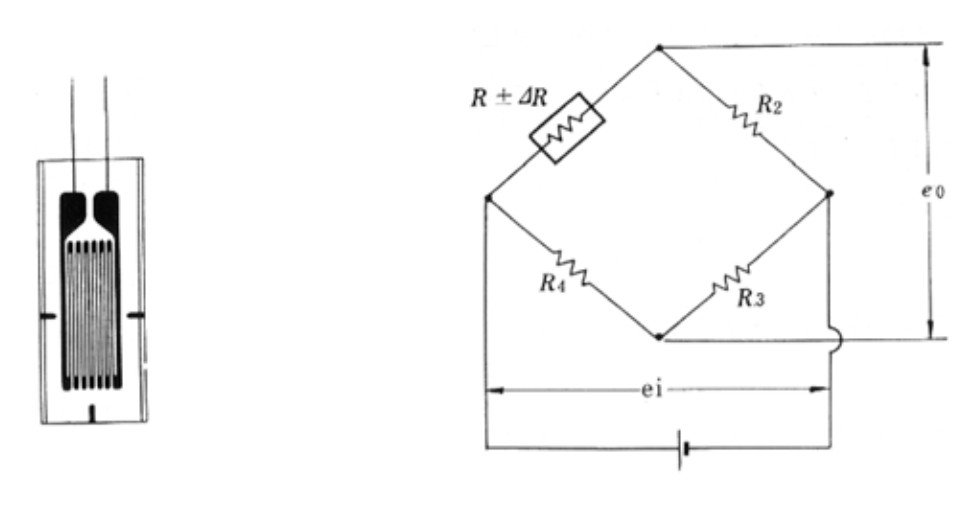
\includegraphics[width=0.6\textwidth]{summer/ship-experiment/tension/pictures/wheatstone.png}
    \caption{ホイートストンブリッジ回路}
    \label{fig:wheatstone}
\end{figure}

\section{手順}
% \usepackage{xcolor} をプリアンブルに追加すれば、{\color{red}テキスト} のように赤字にできるよ
\subsection{事前準備}
\begin{enumerate}
    \item 記録係兼指揮者1名、PC操作係1名、アンプ操作係1名、チャッキング作業補助者2名、試験片計測・ゲージ接続係2\textasciitilde3名を選んだ。
    \item 試験片材料の規格・名称をミルシートから転記し、アンプ ch1\textasciitilde ch2 の結線を記録した。
    \item アンプ ch1\textasciitilde ch2 の計測レンジ、CAL レンジを記録した。
    \item ノギスにより、丸棒試験片平行部の直径を測定して原断面積 $A_0$ を算出した。
\end{enumerate}

\subsection{アンプ CAL 実施}
\begin{enumerate}
    \item アンプのBAL ボタンを押した。
    \item ソフトの「収録開始」ボタンをクリックした。
    \item アンプのCAL レバーを上に押して数秒間ホールドし、離した。
    \item アンプのCAL レバーを下に押して数秒間ホールドし、離した。
    \item ソフト画面の「停止」ボタンをクリックした。
    \item 計測データをCSV形式でPCに保存した。
\end{enumerate}

\subsection{引張り試験実施}
\begin{enumerate}
    \item 計測ソフトを計測待機状態にした。
    \item アンプのBAL ボタンを押した。
    \item 指揮者の合図を受けて、「収録開始」ボタンをクリックした。
    \item 試験片がくびれ、破断する様子を観察した。
    \item 試験片破断後、指揮者の合図を受けて、「停止」ボタンをクリックした。
    \item 計測データをCSV形式でファイルに保存した。
\end{enumerate}

\section{結果}
\subsection{データ処理の方法}
本章では、取得したデータから各種物理量を算出する方法と、その結果について述べる。

\subsection{試験片計測}
使用した試験片はJIS 14A号試験片である。平行部の直径を3箇所で3回ずつ測定した。
\begin{table}[H]
    \centering
    \caption{試験片直径の測定結果 (mm)}
    \begin{tabular}{|l|c|c|c|c|}
        \hline
         & 1回目 & 2回目 & 3回目 & 平均 \\ \hline
        上端 & 12.25 & 12.10 & 11.90 & 12.083 \\ \hline
        中央 & 12.20 & 12.20 & 12.00 & 12.133 \\ \hline
        下端 & 12.23 & 12.10 & 12.00 & 12.110 \\ \hline
    \end{tabular}
\end{table}


9回の測定値の平均は 12.109 mm であった。これより原断面積 $A_0$ は次のように計算される。
$$
A_0 = \pi \left( \frac{12.109}{2} \right)^2 \approx 115.159 \ (mm^2)
$$

\subsection{Cal データからの $\frac{d\epsilon}{dV}$ の算出}
Calデータから、各チャンネルでの1Vの電圧変動に対する歪変化量を算出する。
\begin{figure}[H]
    \centering
    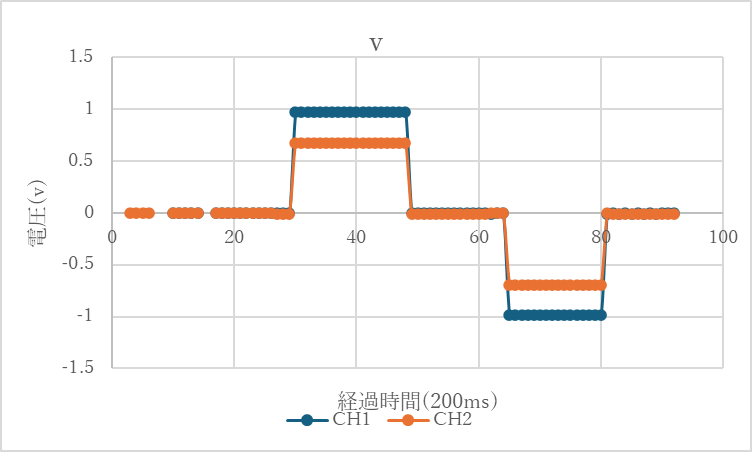
\includegraphics[width=0.8\textwidth]{summer/ship-experiment/tension/pictures/cal_voltage.png}
    \caption{Calデータの電圧分布}
    \label{fig:cal_voltage}
\end{figure}


$\frac{d\epsilon}{dV}$ は以下の式から得られる。
$$
\frac{d\epsilon}{dV} = \frac{2 \times (\text{CAL Range})}{V_{pp}}
$$
\begin{table}[H]
    \centering
    \caption{$\frac{d\epsilon}{dV}$ の算出結果}
    \begin{tabular}{|c|c|c|c|}
        \hline
        CH & 計測レンジ & CAL レンジ & $d\epsilon/dV$ \\ \hline
        CH1 & 5000 & 5000 & 5103.06 \\ \hline
        CH2 & 5000 & 5000 & 7299.88 \\ \hline
    \end{tabular}
\end{table}

\subsection{ひずみ増分 $\Delta \epsilon (t)$ の算出}
引張試験計測データと4.3で得た $\frac{d\epsilon}{dV}$ から、ひずみ増分 $\Delta \epsilon (t)$ を算出する。
\begin{figure}[H]
    \centering
    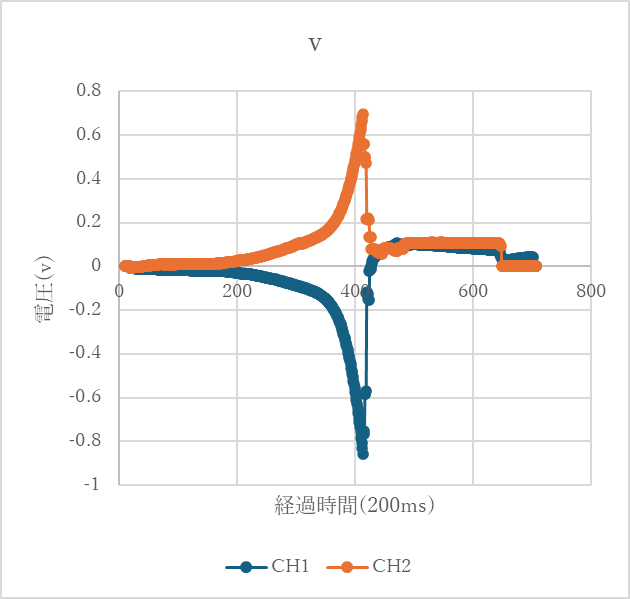
\includegraphics[width=0.8\textwidth]{summer/ship-experiment/tension/pictures/strain_voltage.png}
    \caption{引張試験時の電圧変化}
    \label{fig:strain_voltage}
\end{figure}
$$
\Delta\epsilon(t) = \frac{d\epsilon}{dV}\Delta V(t)
$$

\subsection{荷重増分 $\Delta P$ の算出}
CH3の電圧変化から荷重増分 $\Delta P$ を算出する。
$$
\Delta P\ [\text{kN}] = C\ [\text{kN/V}] \cdot \Delta E\ [\text{V}]
$$
係数 C は最大荷重 68.55 kN の時に 5V となることから、 $C=13.71$ kN/V とした。
\begin{figure}[H]
    \centering
    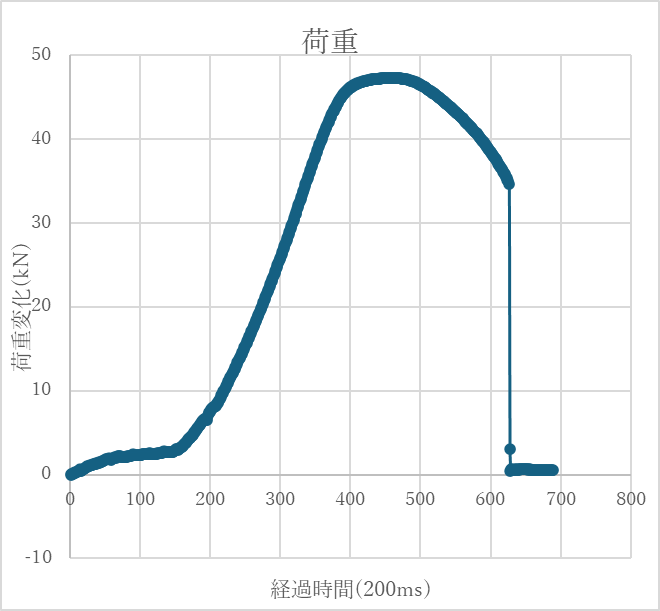
\includegraphics[width=0.8\textwidth]{summer/ship-experiment/tension/pictures/load_change.png}
    \caption{荷重の時間変化}
    \label{fig:load_change}
\end{figure}

\subsection{公称応力-ひずみ関係}
算出した荷重を原断面積で除して公称応力を得て、ひずみとの関係をプロットした。
\begin{figure}[H]
    \centering
    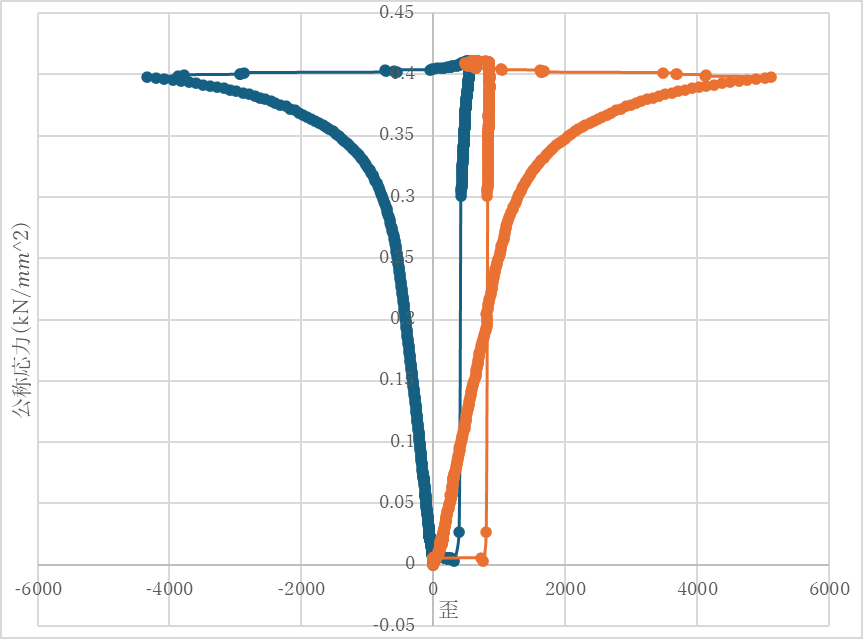
\includegraphics[width=0.8\textwidth]{summer/ship-experiment/tension/pictures/stress_strain.png}
    \caption{公称応力とひずみの関係}
    \label{fig:stress_strain}
\end{figure}

\subsection{ヤング率とポアソン比の算出}
応力-ひずみ関係のグラフの弾性変形区間の傾きからヤング率を算出した。
\begin{table}[H]
    \centering
    \caption{ヤング率の算出}
    \begin{tabular}{|c|c|c|c|c|c|}
        \hline
         & x1 & y1 & x2 & y2 & $E\ (kN/mm^2)$ \\ \hline
        CH1 & 0 & 0 & -250.05 & 0.1206 & -482.30 \\ \hline
        CH2 & 0 & 0 & 503.69 & 0.1206 & 239.43 \\ \hline
    \end{tabular}
\end{table}


CH1が縦ひずみ、CH2が横ひずみであったと仮定すると、ポアソン比 $\nu$ は次式により 1.852 と算出される。
$$
\nu = \left| \frac{\Delta\epsilon_{t}}{\Delta\epsilon_{L}} \right|
$$

\subsection{0.2\%耐力と引張強さ}
本実験では明瞭な降伏点が現れなかったため、0.2\%耐力を算出した。ひずみが0.2\% (2000 $\mu \epsilon$) となった点での公称応力は 0.3688 $kN/mm^2$ であった。
最大荷重は 68.55 kN であったので、引張強さは $0.5953\ kN/mm^2$ となる。

\section{考察}
\subsection{Cal データについて}
CH1とCH2の電圧差が大きく、歪ゲージの設置かホイートストンブリッジ回路に問題がある可能性がある。特に、半田付けの際に以前から付着していた半田を溶かして再溶接したため、その部分にごみが溜まる等で抵抗になっていた事が考えられる。

\subsection{縦歪と横歪の符号について}
縦ひずみが負、横ひずみが正となっており、引張の様子を考えればこれは逆である。また、4.7で算出したポアソン比が1を超えていることからも、CH1とCH2を逆に接続していたと考えられる。
CH1を横ひずみ、CH2を縦ひずみとしてポアソン比を再計算すると、
$$
\nu = \left| \frac{-250.05}{503.69} \right| \approx 0.496
$$
となり、現実的な値となった。
この仮定に基づくと、ヤング率はCH2の値である 239.43 $kN/mm^2$ が妥当であり、0.2\%耐力はCH2のひずみが0.2\%となった点の応力である 0.3476 $kN/mm^2$ となる。

\subsection{ヤング率について}
CH2から算出したヤング率は$239.43kN/mm^2$であった。軟鋼の一般的な縦弾性係数の文献値は約 $206 kN/mm^2$であり、これと比較すると約16\%
大きい値となった。この誤差の原因としては、グラフの弾性域から傾きを読み取る際の区間の取り方や、ひずみゲージの接着状態による測定誤差などが考えられる。

\begin{thebibliography}{99}
    \bibitem{ref1} 授業資料: 引張り 2025-実験の手引き
    \bibitem{ref2} 高橋幸伯, 町田進, 角洋一. 基礎材料力学[三訂版]
    \bibitem{ref3} MiSUMi ホームページ: \UrlFont{https://jp.misumi-ec.com/}
\end{thebibliography}
\end{document}